%%%%%%%%%%%%%%%%%%%%%%%%%%%%%%%%%%%%%%%%%%%%%%%%%%%%%%%%%%%%%%%%%%
%%	  mmm  mmmmmm mm   m        m    m mmmmmm  mmmm				%%
%%	m"   " #      #"m  #        #    # #      #    #			%%
%%	#   mm #mmmmm # #m #        #    # #mmmmm "mmmm"			%%
%%	#    # #      #  # #  """   #    # #      #   "#			%%
%%	 "mmm" #mmmmm #   ##        "mmmm" #mmmmm "#mmm"			%%
%%							      								%%
%%                                                              %%
%%                                                              %%
%%      Grundlagen der Elektrischen Netzwerke, UE               %%
%%      Gruppe 5, Team F                                        %%
%%      Authors: Severin Wolf, Maximilian Seidler.              %%
%%%%%%%%%%%%%%%%%%%%%%%%%%%%%%%%%%%%%%%%%%%%%%%%%%%%%%%%%%%%%%%%%%
\documentclass[a4paper]{article}
\usepackage{amsmath}
\usepackage[utf8]{inputenc}
\usepackage[T1]{fontenc}
\usepackage[english]{babel}
\usepackage{geometry}
\usepackage{graphicx}
\usepackage{tikz}
\usepackage{listings}
\usepackage{trfsigns}
\geometry{a4paper,left=3cm,right=2cm, top=2cm, bottom=2cm} 
\usepackage[EFvoltages, european, straightvoltages]{circuitikz}

%tikz
\ctikzset{resistor = european}
\usetikzlibrary{decorations.pathreplacing}

%no paragraph indent
\setlength{\parindent}{0pt}

%for math, that does not fit
\renewcommand*{\arraystretch}{1.3}
\newcommand\scalemath[2]{\scalebox{#1}{\mbox{\ensuremath{\displaystyle #2}}}}

\newcommand\blfootnote[1]{%
	\begingroup
	\renewcommand\thefootnote{}\footnote{#1}%
	\addtocounter{footnote}{-1}%
	\endgroup
}

% upright differenzial symbol with good spacing included!!!
\makeatletter
\providecommand*{\diff}%
	{\@ifnextchar^{\DIfF}{\DIfF^{}}}
\def\DIfF^#1{%
	\mathop{\mathrm{\mathstrut d}}%
		\nolimits^{#1}\gobblespace
}
\def\gobblespace{%
	\futurelet\diffarg\opspace}
\def\opspace{%
	\let\DiffSpace\!%
	\ifx\diffarg(%
		\let\DiffSpace\relax
	\else
		\ifx\diffarg\{%
			\let\DiffSpace\relax
		\else
			\ifx\diffarg\{%
				\let\DiffSpace\relax
			\fi\fi\fi\DiffSpace}

\begin{document}
\pagestyle{empty} \enlargethispage*{25cm}\samepage{
\vspace*{-3cm}
\begin{center}
\begin{minipage}[!h]{16cm}
\hspace*{0.2cm}

\includegraphics[width=3.3cm]{./Figures/igte_logo}
\begin{tabular}{p{8cm}}
\vspace{0.2cm}
\centering{
\Large Institute of Fundamentals and Theory in
 Electrical Engineering\\
Graz University of Technology\\
~\\}
\end{tabular}

\includegraphics[width=3.3cm]{./Figures/TUG_logo}
\end{minipage}
		\Large
		\textbf{Electric Circuits and Multiports} \vspace*{0.5cm}\\
		\textbf{8. Homework}\\Laplace Transform
		\vspace*{0.5cm}
		
		\large
		13 May 2021
	\end{center}}
	\vspace*{1cm}
	%%%%%%%%%%%%%%%%%%%%%%%%%%%%%%%%%%%%%%%%%%%%%%%%%%%%%%%%%%%%%%%%%%%%
	%%%%%%%%%%%%%%%%%%%%%%%%%%%%%%%%%%%%%%%%%%%%%%%%%%%%%%%%%%%%%%%%%%%%
	\section*{Assignment 1: Node-Voltage Method (2P)}
	The Laplace-Transform as well as the modified node voltage method should be used for the following circuit analysis:
	
	\begin{enumerate}
		\item Transform the input voltage $u_S(t)$ to the $s$-domain: (\textbf{0.25 Points})
		\begin{equation*}
		u_S(t)= U_0 \cdot \sin(\omega t)
		\end{equation*}
		\item Derive the $s$-domain equivalent circuit. The possibility of initial values should be taken into account. The initial conditions are given as: (\textbf{0.5 Points}) 		
		\begin{align*}
			u_{C}(t=0) &= U_{C0}\\
			i_{L2}(t=0) &= I_{L0,2}\\
			i_{L1}(t=0) &= 0~\text{A}
		\end{align*}
		\textbf{ Hint:} Consider which representation of the elements is more suited for the node voltage method.
		\item Apply the node voltage method to the $s$-domain equivalent circuit and write the system of equations in matrix form $A\cdot x = b$. The matrix should be set up by \textbf{closely inspecting} the transformed circuit. Use the \textbf{given node numbers} and the \textbf{reference node}. (\textbf{0.5 Points})
		\item Solve the system of equations in \textit{Matlab} and plot the signals $u(t)$ and $u_C(t)$ for $0\leq t\leq 20ms$. \\(\textbf{0.5 Points}) \\
		\textbf{Hint:} useful \textit{Matlab} commands: \textbf{impulse, minreal, zpk} (lecture 7)...
		\item Explain the difference between frequency domain and Laplace domain in a few sentences.\\(\textbf{0.25 Points})
	\end{enumerate}
\pagebreak
\subsection*{Values:}
$R_1 = 8~\Omega$ \qquad $R_2 = 2~\Omega$ \qquad $R_3 = 2~\Omega$ \qquad $L_1=6~\text{mH}$ \qquad $C=450~\mu\text{F}$ \qquad $L_2=3~\text{mH}$ \qquad $U_0 = 15~\text{V}$ \qquad $\omega = 1000~s^{-1}$ \qquad
$U_{C0} = 1~\text{V}$ \qquad $I_{L0,2} = 1~\text{A}$ \\


 \begin{figure}[h!]
	\centering
		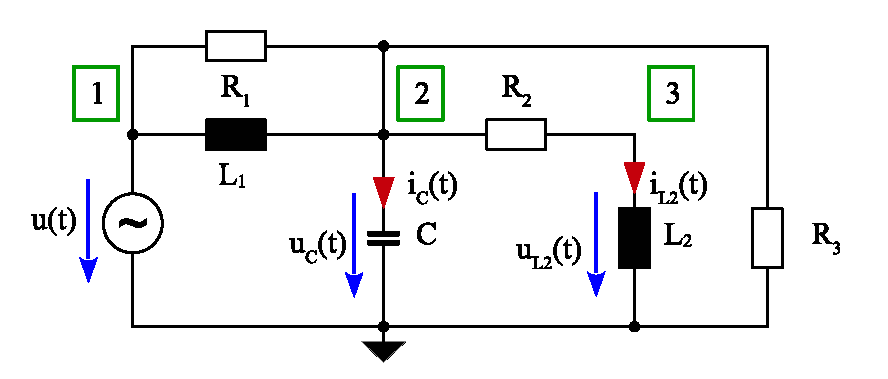
\includegraphics[scale=0.8]{Figures/homework8_circuit_1.eps}
		\caption{Given circuit for assignment 1}
		\label{fig:ass_1}
\end{figure}

	\section*{Assignment 2: Analytical  calculations in Laplace domain (3P)}
The Laplace-Transform should be used for the following circuit analysis:
\begin{enumerate}
	\item Transform the input voltage $u_S(t)$ (DC source) to the $s$-domain: (\textbf{0.25 Points})
	\begin{align*}
	u_S(t)&= U_0\\
	U_s(s) &= \mathcal{L}\{u(t)\}
	\end{align*}
	\item Derive the $s$-domain equivalent circuit. \textbf{Therefore all initial conditions are 0}.(\textbf{0.5 Points}) 
	\item Determine the expression for $U_L(s) = \mathcal{L}\{u_L(t)\}$ in the s-domain. 
	\begin{itemize}
	\item Use a voltage divider in order to obtain the expression for $\frac{U_L(s)}{U_s(s)}$. (\textbf{0.75 Points})
	\item Derive an expression for $U_L(s)$ of the following form: (\textbf{0.5 Points})
	\begin{align*}
		U_L(s) = K\cdot \frac{s+d}{s^2+s\cdot 2a+b}
	\end{align*}
	and calculate the values of $K$, $a$, $b$ and $d$. \textbf{Hint:} these substitutions ($K$, $a$, $b$ and $d$) can be used in further calculations from this point on.
	\end{itemize}
	\item Find the time-domain expressions for the voltage $U_L(s) = \mathcal{L}\{u_L(t)\}$. \\
	\textbf{Hint:} partial fraction expansion is not required. Check out the known transformations from lecture 7. (\textbf{0.5 Points})
	\item Plot the voltage $u_L(t)$ in \textit{Matlab} and confirm the result by simulating the circuit in LTspice.\\(\textbf{0.5 Points})
\end{enumerate}
\pagebreak
\subsection*{Values:}
$R_1 = 8~\Omega$  \qquad $L=15~\text{mH}$ \qquad $C=60~\mu \text{F}$ \qquad $U_0 = 15~\text{V}$ \\
\begin{figure}[h!]
	\centering
	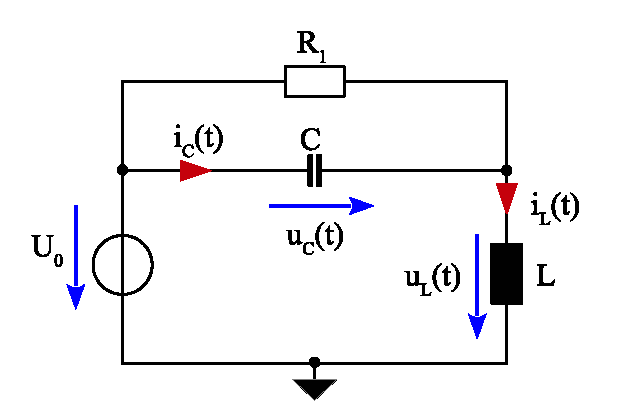
\includegraphics[scale=0.8]{Figures/homework8_circuit_2.eps}
	\caption{Given circuit for assignment 2}
\end{figure}







\section*{voluntary - Bonus example for the second exam - 0P}

This is a bonus example for the second exam in order to gain some practice. \\
It's voluntary, but I'll correct it if handed in. \\
\vspace*{1cm}

Consider the given circuit in figure \ref{fig:homework8circuitbonus}. 

\begin{enumerate}
	\item Derive the $s$-domain equivalent circuit. The possibility of initial values should be taken into account.
	\item Transform the input voltage $u(t)$ to the $s$-domain:
	\begin{equation*}
	u(t)= U_0 
	\end{equation*}
	\item Simplify the given circuit by setting the initial condition $u_C(t = 0) = U_{C,0} = 0V$. 
	\item Find the expression for $U_C(s) = \mathcal{L} \{u_c(t)\}$.
	\item Find the expression for $I_C(s) = \mathcal{L} \{i_c(t)\}$.
	\item Derive the expression for $i_c(t)$ and $u_c(t)$.
\end{enumerate}

\pagebreak
\subsection*{Values:}
$R_1 = 10~\Omega$ \qquad $R_2 = 4~\Omega$ \qquad $R_3 = 50~\Omega$ \qquad $C=500~\mu F$ \qquad $U_0 = 10~V$ \\

\begin{figure}[!htp]
	\centering
	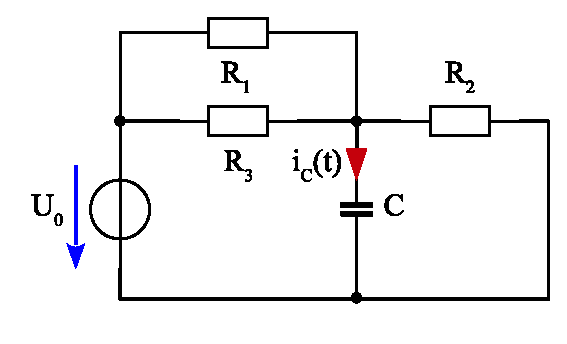
\includegraphics[width=0.55\linewidth]{Figures/homework8_circuit_3}
	\caption{Given circuit for the bonus example}
	\label{fig:homework8circuitbonus}
\end{figure}

\blfootnote{Submission deadline: 27 May 2021; \qquad Presentation: Team 8}

\pagebreak

\section{Solution assignment 1}
\subsection{Analytical solution}
Transform the input voltage to the s-domain, like such:
\[
  u_s(t) = U_{0} \cdot \sin(\omega t) \quad\laplace\quad U_{s}(s) = U_0 \cdot \frac{\omega}{s^2 +\omega^2}
.\] 
The laplace domain equivalen for the circuit in figure \ref{fig:ass_1}. We use paralell current
sources, that represent our initial conditions in the laplace domain, because they will become a
constant term on the right side of our node voltage equation $A\vec{x} = \vec{b}$. Because the
initial Condition at $L_1$ is equal to $0A$, the laplace domain equivalent of $L_1$ does not need a
additional source.
\begin{figure}[!ht] \centering 
  \begin{circuitikz}[scale=0.85, transform shape]
    \draw (0,0) to[sV=$U_s(s)$, i>=$I_{U}^{?}(s)$] (0,5)
    (0,5) to[L=$sL_1$, *-*, i=$I_{L1}(s)$, v=$sL_1 I_{L1}(s)$] (5,5)
    (5,5) to[C=$\frac{1}{sC}$, -*, i=$I_{C}(s)$, v=$\frac{I_{C}(s)}{sC}$] (5,0)
	  (5,5) to[short] (7,4) 
	  (7,1) to[isource=$CU_{C0}$] (7,4)
	  (7,1) to[short] (5,0)
	  (5,5) to[R=$R_2$, i=$I_{R2}(s)$, v=$R_2 I_{R2}(s)$] (10,5)
	  (10,5) to[L, l=$sL_2$, -*, i=$I_{L2}(s)$, v=$sL_2 I_{L2}(s)$] (10,0)
	  (10,5) to[short, *-] (12,4)
	  (12,4) to[isource=$\frac{i_{L0,2}}{s}$] (12,1)
	  (12,1) to[short] (10,0)
	  (0,0) to[short] (15,0)
	  (15,0) to[R=$R_3$, i<=$I_{R3}(s)$, v<=$R_3 I_{R3}(s)$] (15,7)
	  (15,7) to[short] (5,7)
	  (5,7) to[short] (5,5)
	  (5,7) to[R=$R_1$, i<=$I_{R1}(s)$, v<=$R_1 I_{C}(s)$] (0,7)
	  (0,7) to[short] (0,5);
	  \node[above, xshift=-3mm, color=blue]	    (n_1) at (0, 5) {$n_1$};
	  \node[above, xshift=3mm, color=blue]	    (n_2) at (5, 5) {$n_2$};
	  \node[above, xshift=3mm, color=blue]	    (n_3) at (10, 5) {$n_3$};
	  \draw[-{Latex[length=2mm]}, color=blue] (0.5, 4.5) -- (2, 0.5)
	  node[pos=0.25, left] {$U_{n_1}$};
	  \draw[-{Latex[length=2mm]}, color=blue] (4.5, 4.5) -- (2.5, 0.5)
	  node[pos=0.25, left] {$U_{n_2}$};
	  \draw[-{Latex[length=2mm]}, color=blue] (8.6, 2.25) -- (7.9, 0.5);
	  \draw[color=blue] (9.5, 4.5) -- (8.8, 2.8)
	  node[pos=0.25, left] {$U_{n_3}$};
	  \draw (0,0) to (0,0) node[ground]{};
  \end{circuitikz}
  \caption{laplace domain circuitikz assignment 1}
  \label{fig:lap_circ}
\end{figure}

 Kirchhoff's current law gets us $3$ nodal equations.
\begin{align*}
  (n_1):&\quad -I_{U}^{?}(s) + I_{R_1}(s) + I_{L1}(s) = 0 \\
  (n_2):&\quad-I_{R1}(s) - I_{L1}(s) +I_{R2}(s) + I_{C}(s) = CU_{C0} \\
  (n_3):&\quad -I_{R2}(s) + I_{L2}(s) = - \frac{i_{L0, 2}}{s}
\end{align*}
From those equations, we could derive the our node voltage equation $A\vec{x} = \vec{b}$, by 
rewriting the currents as nodal voltages divided by laplace domain impedances.
However, since we know how that works, the standard admittance matrix $A$ is determined by
inspection. 
\[
  \begin{pmatrix}
    \frac{1}{R_1} + \frac{1}{sL_1} & -\frac{1}{R_1} - \frac{1}{sL_1} & 0 \\
    -\frac{1}{R_1} - \frac{1}{sL_1} & \frac{1}{R_1} + \frac{1}{R_2} + \frac{1}{R_3} + 
    \frac{1}{sL_1} + sC & -\frac{1}{R_2} \\ 
    0 & -\frac{1}{R_2} & \frac{1}{R_2} + \frac{1}{sL_2}
  \end{pmatrix}
.\] 
The vector $\vec{x}$ contains the unkown values of our circuit. Since there is a voltage source in
our circuit, we need the current  $I_{U}^{?}(s)$ to be in that vector as well.
\[
  \vec{x} =
  \begin{pmatrix}
    U_{n1} \\ U_{n2} \\ U_{n3} \\ I_{U}^{?}(s) 
  \end{pmatrix}
.\] 
The get a solvable system of linear equations, we need an additional equation, which brings the
voltage source $U_s(s)$ (Figure \ref{fig:lap_circ}) into context. This context is given via 
$U_s(s) = -U_{n1}$. With the vector $\vec{b}$, which contains the values of all sources in Figure
\ref{fig:lap_circ}, we get:
\[
  \begin{pmatrix}
    \frac{1}{R_1} + \frac{1}{sL_1} & -\frac{1}{R_1} - \frac{1}{sL_1} & 0 & -1\\
    -\frac{1}{R_1} - \frac{1}{sL_1} & \frac{1}{R_1} + \frac{1}{R_2} + \frac{1}{R_3} + 
    \frac{1}{sL_1} + sC & -\frac{1}{R_2} & 0\\ 
    0 & -\frac{1}{R_2} & \frac{1}{R_2} + \frac{1}{sL_2} & 0 \\
    -1 & 0 & 0 & 0
  \end{pmatrix} \cdot
  \begin{pmatrix}
    U_{n1} \\ U_{n2} \\ U_{n3} \\ I_{U}^{?}(s)  
  \end{pmatrix} =
  \begin{pmatrix}
    0 \\ CU_{C0} \\ - \frac{I_{L0,2}}{s} \\ U_s(s)
  \end{pmatrix}
.\] \clearpage
Bevor we will solve that system in matlab and plot the results (section \ref{sec:matlab}), 
let's quickly assess some differences between the frequency domain and the laplace domain.
\bigskip
\\The most important thing, that the laplace domain gives us, is a transformed space, where
derivations become multiplications and integrations divisions. That enables us, to treat passiv
elements like capacitors and inductors as if they had a linear relation between their voltages and
currents. That's why we can apply the node voltage method, to calculate a transient response with a 
sinusoidal input, only using a linear system of equations.
\subsection{Matlab} \label{sec:matlab}
\subsubsection{Output}
With the source code shown in section \ref{sec:source}, we generated the following plot (Figure
\ref{fig:matl_ass1}),
that shows $u_{s}(t)$ and $u_{C}(t)$, witch correspond to the nodevoltages like such: $u_{s}(t) = -u_{n1}(t)$
and $u_{C}(t) = u_{n2}$.
\begin{figure}[ht]
  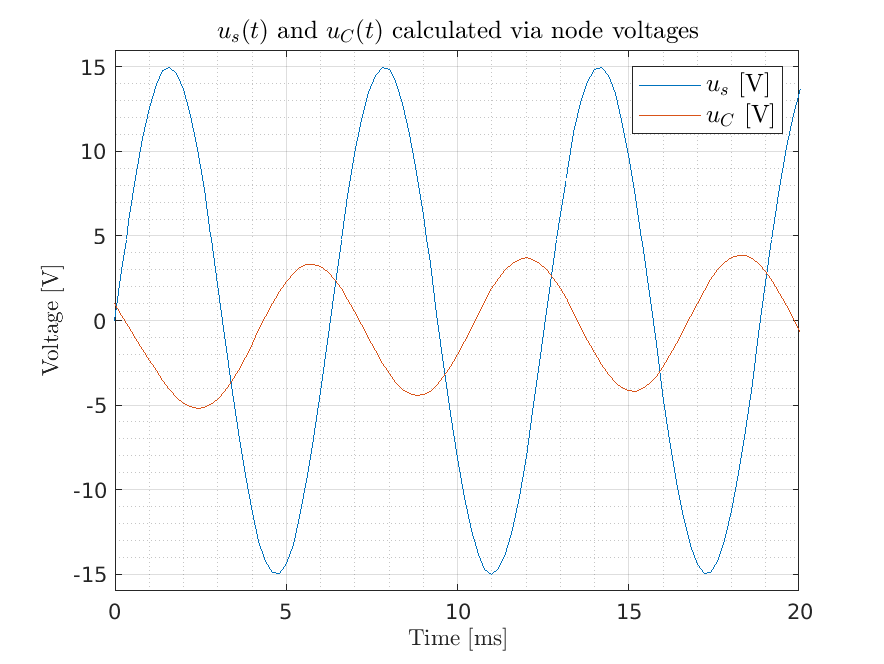
\includegraphics{./Figures/ue8_ass_1_plot.png}
  \caption{matlab plot assignment 1}
  \label{fig:matl_ass1}
\end{figure}

\subsubsection{Source code} \label{sec:source}
\lstinputlisting[language=matlab]{./../matlab/UE8_1.m}

\pagebreak

\section{Solution assignment 2}
\subsection{Transformation of $u_s(t)$}

\begin{align*}
	U_0 \;\;\; \laplace \;\;\; \frac{15}{s}
\end{align*}

\subsection{Transformation of the Network}
As all initial conditions are zero, we do not need to take them into consideration and can simply transform the network into the s-domain.

\begin{figure}[!h] \centering
	\begin{circuitikz}
		\draw (0,1)
		to[V, v<=$U_0$](0,5)
		to[short, *-](0,7)
		to[R, l=$R_1$](5,7)
		to[short, -*](5,5)
		to[short, i=$I_L(s)$, color=red](5,4)
		to[L, l=$sL$, v=$U_L(s)$](5,1)
		to[short, -*](0,1);
		\draw(0,5)
		to[short, i=$I_C(s)$, color=red](1,5)
		to[C, l=$\frac{1}{sC}$, v=$U_C(s)$](4,5)
		to[short, -*](5,5);
		\draw (0,1) node[ground]{};
	\end{circuitikz}
\end{figure}

\subsection{Determination of $U_L(s)$}
In order to find $U_L(s)$ we use a volatge divider:
\begin{equation*}
	\frac{U_L(s)}{U(s)} = \frac{sL}{\frac{R_1 \cdot \frac{1}{sC}}{R_1 + \frac{1}{sC}} + sL}\\
\end{equation*}
\\
\begin{align*}
	U_L(s) = U(s) \cdot \frac{sL}{\frac{R_1 \cdot \frac{1}{sC}}{R_1 + \frac{1}{sC}} + sL} = 
	U(s) \cdot \frac{sL}{\frac{R_1 \cdot \frac{1}{sC} + sL(R_1 + \frac{1}{sC})}{R_1 + \frac{1}{sC}}} = 
	U(s) \cdot \frac{sL(R_1 + \frac{1}{sC})}{R_1 \cdot \frac{1}{sC} + sL(R_1 + \frac{1}{sC})} =
	U(s) \cdot \frac{sLR_1 + \frac{L}{C}}{\frac{R_1}{sC} + sLR_1 + \frac{L}{C})} =\\
	U(s) \cdot \frac{sLR_1 + \frac{L}{C}}{\frac{R_1 + s^2LCR_1 + sL}{sC}} =
	\frac{U_0}{s} \cdot \frac{s^2LCR_1 + sL}{R_1 + s^2LCR_1 + sL} =
	U_0 \cdot \frac{sLCR_1 + L}{s^2LCR_1 + sL + R_1} =
	U_0 \cdot \frac{s + \frac{1}{CR_1}}{s^2 + s \cdot \frac{1}{CR_1} + \frac{1}{LC}}
\end{align*}
We substitute to the form
\begin{equation*}
	U_L(s) = K\cdot \frac{s+d}{s^2+s\cdot 2a+b}
\end{equation*}
with $K = U_0$, $a = \frac{1}{2CR_1}$, $b = \frac{1}{LC}$ and  $d = \frac{1}{CR_1}$.
\begin{align*}
	K &= 15,& a &= 1041.6,& b &= 1.111 \cdot 10^{6},& d &= 2083,3
\end{align*}

\pagebreak

\subsection{Retransformation into time domain}
$s^2 + 2as + b$ has complex zeros, so we use the transformations of sin and cos:
\begin{align*}
	e^{-at}\cos(\omega t)\;\;\; &\laplace \;\;\; \frac{s+a}{(s+a)^2 + \omega^2},&
	e^{-at}\sin(\omega t)\;\;\; &\laplace \;\;\; \frac{\omega}{(s+a)^2 + \omega^2}
\end{align*}

In order to do that we nee to bring the upper equation into the correct form.
\begin{align*}
	U_L(s) = K\cdot \frac{s+d}{s^2+s\cdot 2a+b} = K\cdot \frac{s+d}{(s+a)^2-a^2+b} = 
	K\cdot \frac{s+a-a+d}{(s+a)^2-a^2+b} =\\
	K\cdot \frac{s+a}{(s+a)^2-a^2+b} + K\cdot \frac{d-a}{(s+a)^2-a^2+b} = 
	K\cdot \frac{s+a}{(s+a)^2-a^2+b} + K\cdot \frac{d-a}{\sqrt{b-a^2}} \cdot \frac{\sqrt{b-a^2}}{(s+a)^2-a^2+b} = 
\end{align*}
Because the laplace-transformation is a linear operation we now can simply transform these two parts.
\begin{align*}
	K\cdot \frac{s+a}{(s+a)^2-a^2+b} \;\;\; &\laplace \;\;\; K\cdot e^{-at}\cos \left(\sqrt{b-a^2}t \right)\\
	K\cdot \frac{d-a}{\sqrt{b-a^2}} \cdot \frac{\sqrt{b-a^2}}{(s+a)^2-a^2+b} \;\;\; &\laplace \;\;\;
	K\cdot \frac{d-a}{\sqrt{b-a^2}} \cdot e^{-at}\sin \left(\sqrt{b-a^2}t \right)\\
	U_L(s) \;\;\; &\laplace \;\;\; K\cdot e^{-at} \left(\cos \left(\sqrt{b-a^2}t \right) + 
	\frac{d-a}{\sqrt{b-a^2}} \cdot \sin\left(\sqrt{b-a^2}t\right) \right)\\
\end{align*}
Now we can plug in the values:
\begin{align*}
	u_L(t) =& 15\cdot e^{-1041.6t} \left(\cos \left(\sqrt{1.111\cdot 10^{6}-1041.6^2}t \right) + 
	\frac{2083,3-1041.6}{\sqrt{1.111\cdot 10^{6}-1041.6^2}} \cdot \sin\left(\sqrt{1.111\cdot 10^{6}-1041.6^2}t\right) \right)\\
\end{align*}
and we get:
\begin{align*}
	u_L(t) =& 15\cdot e^{-1041.6t} \left(\cos(161.4t) + 
	6.455 \cdot \sin\left(161.4t\right) \right)\\
\end{align*}

\subsection{Simulations and plots}
\subsubsection{Matlab}
\lstinputlisting[language=matlab]{./../matlab/assignment8_2.m}

\begin{figure}[h!]\centering
	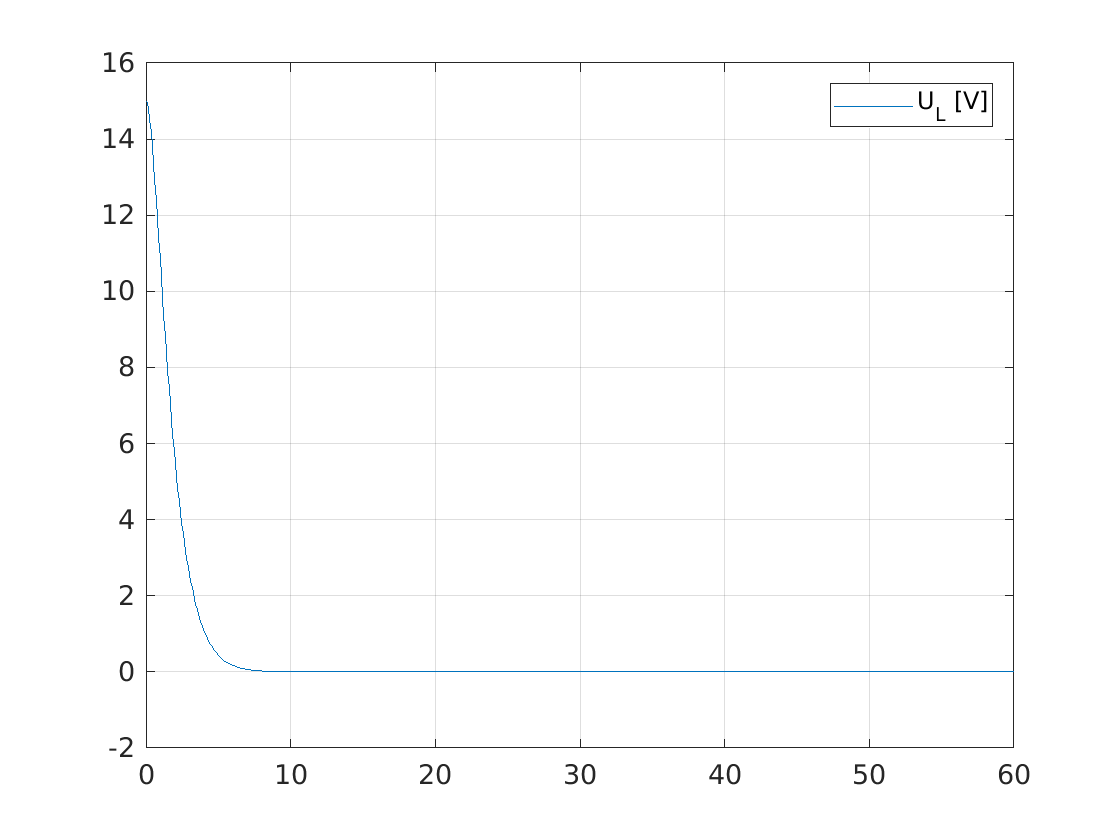
\includegraphics[scale=0.7]{./../matlab/graph.png}
	\caption{Matlab simulation result}
\end{figure}
\pagebreak

\subsubsection{LTspice}

\begin{figure}[h!]\centering
	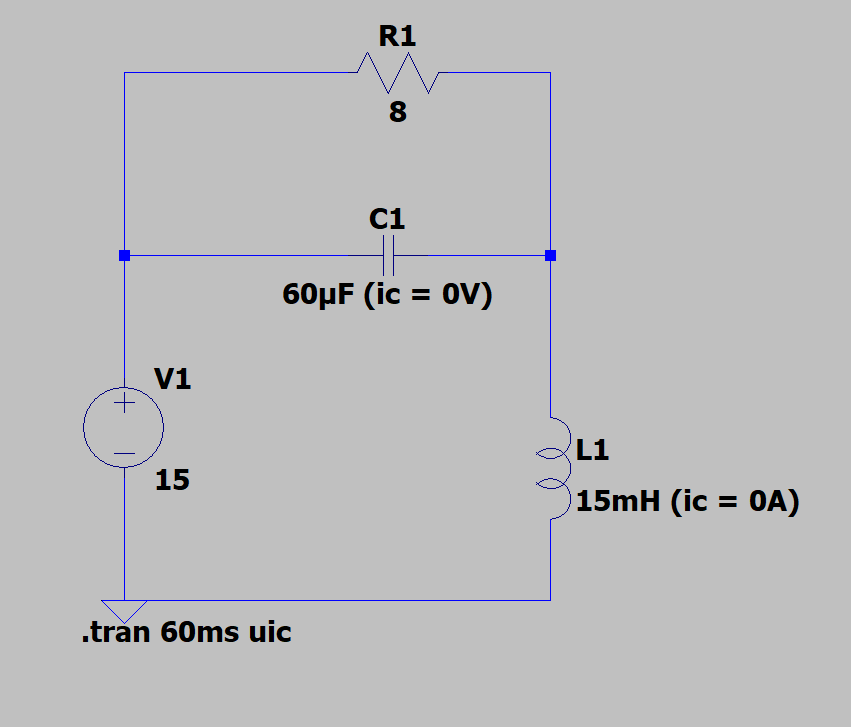
\includegraphics[scale=0.5]{./../LTspice/Assignment2.PNG}
	\caption{LTspice simulation}
\end{figure}

\begin{figure}[h!]\centering
	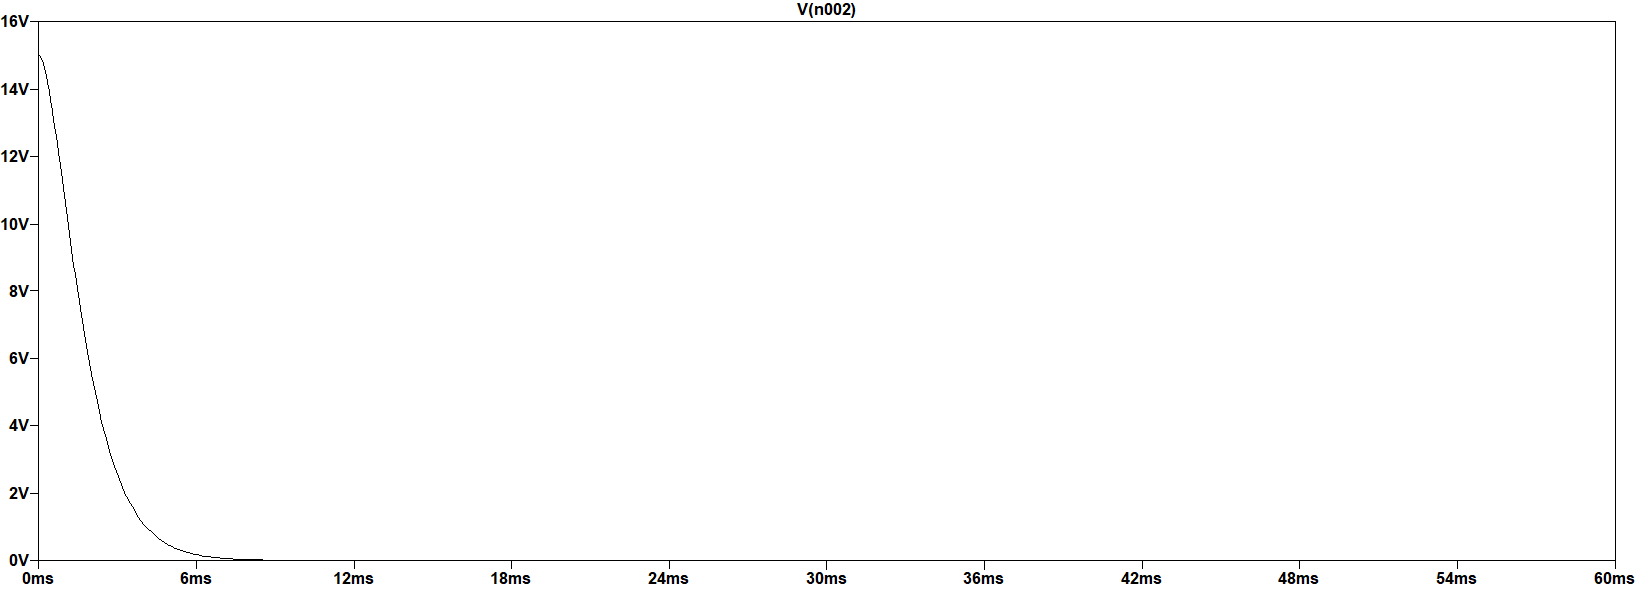
\includegraphics[scale=0.4]{./../LTspice/Assignment2_plot.png}
	\caption{LTspice simulation result}
\end{figure}

\end{document}
